%------------------------------------------------------------------------------
% CV in Latex
% Author : Charles Rambo
% Based off of: https://github.com/sb2nov/resume and Jake's Resume on Overleaf
% Most recently updated version may be found at https://github.com/fizixmastr 
% License : MIT
%------------------------------------------------------------------------------

% \documentclass[A4,11pt]{article}
\documentclass[letterpaper,11pt]{article} %For use in US
\usepackage{latexsym}
\usepackage[empty]{fullpage}
\usepackage{titlesec}
\usepackage{marvosym}
\usepackage[usenames,dvipsnames]{color}
\usepackage{verbatim}
\usepackage{enumitem}
% \usepackage[hidelinks]{hyperref}
\usepackage[english]{babel}
\usepackage{tabularx}
\usepackage{tikz}
% \usepackage{changes}
% \usepackage{bibentry}
\usepackage{bibentry}
\makeatletter\let\saved@bibitem\@bibitem\makeatother
\usepackage{hyperref}
\makeatletter\let\@bibitem\saved@bibitem\makeatother
% \usepackage{enumitem}
% \usepackage{biblatex}
\input{glyphtounicode}

% \nobibliography{publications}

\begin{comment}
I am by no means a professional when it comes to the CV's/resumes, I have
received various trainings on how to write a CV and resume from my high 
school, as well as the Austin College and University of Eastern Finland's
career counseling departments. As I intend to share my CV as a template, I 
feel that it is my responsibility to provide explanations of my work.
\end{comment}


%-----FONT OPTIONS-------------------------------------------------------------
\begin{comment}
The font of the document will impact not just how readable it is, but how it is
perceived. In the "The Craft of Scientific Writing" by Michael Alley, shares a
common fonts for publication as well as their use. I have chosen to use
Palatino for its legibility, some others are given below. There is far too much
about typography to discus here. Note: serif fonts have short projecting
strokes, sans-serif fonts are sans (without) these strokes.
\end{comment}


% serif
 \usepackage{palatino}
% \usepackage{times} %This is the default as well
% \usepackage{charter}

% sans-serif
% \usepackage{helvet}
% \usepackage[sfdefault]{noto-sans}
% \usepackage[default]{sourcesanspro}

%-----PAGE SETUP---------------------------------------------------------------

% % Adjust margins
% \addtolength{\oddsidemargin}{-1cm}
% \addtolength{\evensidemargin}{-1cm}
% \addtolength{\textwidth}{2cm}
% \addtolength{\topmargin}{-1cm}
% \addtolength{\textheight}{2cm}

% Margins for US Letter size
\addtolength{\oddsidemargin}{-0.5in}
\addtolength{\evensidemargin}{-0.5in}
\addtolength{\textwidth}{1in}
\addtolength{\topmargin}{-.5in}
\addtolength{\textheight}{1.0in}

\urlstyle{same}

\raggedbottom
\raggedright
\setlength{\tabcolsep}{0cm}

% Sections formatting
\titleformat{\section}{
  \vspace{-4pt}\bfseries\raggedright\large
}{}{0em}{}[\color{black}\titlerule \vspace{-5pt}]

% Ensure that .pdf is machine readable/ATS parsable
\pdfgentounicode=1

%-----CUSTOM COMMANDS FOR FORMATTING SECTIONS----------------------------------
\newcommand{\CVItem}[1]{
  \item\small{
    {#1 \vspace{-2pt}}
  }
}

\newcommand{\CVSubheading}[4]{
  \vspace{-2pt}\item
    \begin{tabular*}{0.97\textwidth}[t]{l@{\extracolsep{\fill}}r}
      \textbf{#1} & #2 \\
      \small#3 & \small #4 \\
    \end{tabular*}\vspace{-7pt}
}

\newcommand{\CVSubSubheading}[2]{
  \vspace{-2pt}\item
    \begin{tabular*}{0.94\textwidth}[t]{l@{\extracolsep{\fill}}r}
      {#1} & \small #2
    \end{tabular*}\vspace{-7pt}
}


% \newcommand{\CVSubSubheading}[2]{
%     \item
%     \begin{tabular*}{0.97\textwidth}{l@{\extracolsep{\fill}}r}
%       \text{\small#1} & \text{\small #2} \\
%     \end{tabular*}\vspace{-7pt}
% }

\newcommand{\CVSubItem}[1]{\CVItem{#1}\vspace{-4pt}}

\renewcommand\labelitemii{$\vcenter{\hbox{\tiny$\bullet$}}$}

\newcommand{\CVSubHeadingListStart}{\begin{itemize}[leftmargin=0.5cm, label={}]}
% \newcommand{\resumeSubHeadingListStart}{\begin{itemize}[leftmargin=0.15in, label={}]} % Uncomment for US
\newcommand{\CVSubHeadingListEnd}{\end{itemize}}
\newcommand{\CVSubSubHeadingListStart}{\begin{itemize}[leftmargin=1.0cm, label={}]}
\newcommand{\CVSubSubHeadingListEnd}{\end{itemize}}
\newcommand{\CVItemListStart}{\begin{itemize}}
\newcommand{\CVItemListEnd}{\end{itemize}\vspace{-5pt}}

\usepackage{times}
%------------------------------------------------------------------------------
% CV STARTS HERE  %
%------------------------------------------------------------------------------
\begin{document}
\nobibliography{publications_visa}
\bibliographystyle{unsrt}
% \bibliographystyle{abbrv}
%-----HEADING------------------------------------------------------------------
\begin{comment}
In Europe it is common to include a picture of ones self in the CV. Select
which heading appropriate for the document you are creating.
\end{comment}

% \begin{minipage}[c]{0.05\textwidth}
% \-\
% \end{minipage}
% \begin{minipage}[c]{0.2\textwidth}
% \begin{tikzpicture}
%     \clip (0,0) circle (1.75cm);
%     \node at (0,-.7) {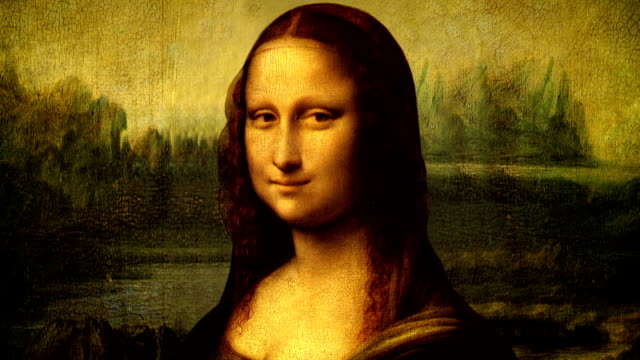
\includegraphics[width = 9cm]{portrait}}; 
%     % if necessary the picture may be moved by changing the at (coordinates)
%     % width defines the 'zoom' of the picture
% \end{tikzpicture}
% \hfill\vline\hfill
% \end{minipage}
% \begin{minipage}[c]{0.4\textwidth}
%     \textbf{\Huge \scshape{Ming Fang}} \\ \vspace{1pt} 
%     % \scshape sets small capital letters, remove if desired
%     \small{+1 217-305-1769} \\
%     \href{mailto:mingf2@illinois.edu}{\underline{mingf2@illinois.edu}}\\
%     % % Be sure to use a professional *personal* email address
%     % \href{https://www.linkedin.com/in/charles-rambo/}{\underline{linkedin.com/in/charles-rambo}} \\
%     % % you should adjust you linked in profile name to be professional and recognizable
%     % \href{https://github.com/fizixmastr}{\underline{github.com/fizixmastr}}
% \end{minipage}

% Without picture
\begin{center}
    \textbf{\Huge Ming Fang} \\ \vspace{1pt} %\scshape sets small capital letters, remove if desired
    % \small 
    +86 13696531002 $|$
    +1 217-305-1769 $|$
    \href{mailto:mingf2@illinois.edu}{{mingf2@illinois.edu}}\\
    {Gender: Male $|$ Date of Birth: Feb 28, 1997}\\
    % {US ADD: 1615 Melrose Park Ct, Apt 2022, Urbana, IL 61801, USA}\\ \vspace{1pt}
    {Address: 9 Wazaoji Road, Yaoxitang Village, Mohuan Township, Longyou County, Quzhou, Zhejiang, China 324400}
    % % % Be sure to use a professional *personal* email address
    % \href{www.linkedin.com/in/ming-fang1}{\underline{linkedin.com/in/ming-fang1}} $|$
    % % you should adjust you linked in profile name to be professional and recognizable
    % \href{https://github.com/fizixmastr}{\underline{github.com/fizixmastr}}
\end{center}






\begin{comment}
This CV was written for specifically for positions I was applying for in
academia, and then modified to be a template.

A standard CV is about two pages long where as a resume in the US is one page.
sections can be added and removed here with this in mind. In my experience, 
education, and applicable work experience and skills are the most import things
to include on a resume. For a CV the Europass CV suggests the categories: Work
Experience, Education and Training, Language Skills, Digital Skills,
Communication and Interpersonal Skills, Conferences and Seminars, Creative Works
Driver's License, Hobbies and Interests, Honors and Awards, Management and
Leadership Skills, Networks and Memberships, Organizational Skills, Projects,
Publications, Recommendations, Social and Political Activities, Volunteering.

Your goal is to convey a who, what , when, where, why for every item you share. 
The who is obviously you, but I believe the rest should be done in that order.
For example below. An employer cares most about the degree held and typically 
less about the institution or where it is located (This is still good 
information though). Whatever order you choose be consistent throughout.
\end{comment}

% \section{Research Interest}
%   \CVItemListStart
%     \CVItem{Development of non-destructive assay methods of special material for the characterization of tri-structural isotropic particle (TRISO) fuel for pebble bed reactors.}
%     \CVItem{Development of single-volume scatter camera with SiPM scintillator readout.}
%     \CVItem{Radiation detector signal processing algorithms with a focus on accelerated Monte Carlo implementation and iterative linear inverse solver for image reconstruction.}
%     \CVItem{Application of advanced radiation detection techniques, such as positron lifetime spectroscopy.}
%   \CVItemListEnd

%-----Research and projects----------------------------------------------------------
\begin{comment}
try to briefly explain what you did and why it is relevant to the position you
are seeking
\end{comment}
\begin{comment}
Ideally the title of the work should speak for what it is. However if you feel
like you should explain more about why the project is applicable to this job,
use item list as is shown in the work experience section.
\end{comment}

\section{Work Experience}
\CVSubHeadingListStart
     \CVSubheading %Example
      {Postdoctoral Research Associate}{Jan. 2024 – Present}
     {University of Illinois Urbana-Champaign}{Urbana, IL, USA}
    \CVItemListStart
        \CVItem{\textbf{Main responsibilities:}  Conduct experiments, organize or analyze data, present findings in a publication}
        \CVItem{\textbf{Main projects and accomplishments:}}
        \begin{enumerate}[leftmargin=0.5cm, nolistsep]
            \item \begin{tabular*}{0.90\textwidth}[t]{l@{\extracolsep{\fill}}r}{Innovated Cover-crop Opportunity, Verification, and Economy stimulating technology\\ for underserved farmers using Robotics} & \small{Jan. 2024 -- Present}\end{tabular*}
            \begin{enumerate}[leftmargin=1.0cm, nolistsep, label=(\roman*)]
                \item Developed an experimental setup to irradiate soil samples with neutron beams
                \item Measured the carbon weight fraction in soil by detecting gamma-rays from neutron-carbon interactions
            \end{enumerate}
        \end{enumerate}
      \CVItemListEnd
%    \CVSubheading % Example
%      {Degree Achieved}{Years of Study}
%      {Institution of Study}{Where it is located}
    \CVSubheading %Example
      {Graduate Teaching Assistant}{Aug. 2023 – Dec. 2023}
     {University of Illinois Urbana-Champaign}{Urbana, IL, USA}
    \CVItemListStart
        % \CVItem{Cumulative GPA:  4.0 / 4.0}
        \CVItem{\textbf{Main responsibilities:} Organize laboratory classes and host office hours.}
        \CVItem{\textbf{Main projects and accomplishments:} None}
      \CVItemListEnd
      
    \CVSubheading
     {Graduate Research Assistant}{Sept. 2018 -- Dec. 2023}
     {University of Illinois Urbana-Champaign}{Urbana, IL, USA}
      \CVItemListStart
        % \CVItem{Cumulative GPA:  4.0 / 4.0}
        \CVItem{\textbf{Main responsibilities:} Conduct experiments, organize or analyze data, present findings in a publication or dissertation}
        \CVItem{\textbf{Main projects and accomplishments:}}
        \begin{enumerate}[leftmargin=0.5cm, nolistsep]
            \item \begin{tabular*}{0.90\textwidth}[t]{l@{\extracolsep{\fill}}r}{Multi-Mode Imaging for TRi-structual ISOtropic (TRISO) Fuel Pebble Identification} & \small{Aug. 2020 -- Dec. 2023}\end{tabular*}
            \begin{enumerate}[leftmargin=1.0cm, nolistsep, label=(\roman*)]
                \item Developed an algorithm to identify fuel pebbles based on X-ray Computed Tomography
            \end{enumerate}
            \item \begin{tabular*}{0.90\textwidth}[t]{l@{\extracolsep{\fill}}r}{Quantitative Image Reconstruction in Passive Gamma Emission Tomography} & \small{Aug. 2019 -- Sept. 2020}\end{tabular*}
            \begin{enumerate}[leftmargin=1.0cm, nolistsep, label=(\roman*)]
                \item Developed an algorithm to reconstruct cross-sectional images of spent nuclear fuel assemblies stored in water pools, identify missing fuel pins, and estimate fuel pin activities
            \end{enumerate}
            \item \begin{tabular*}{0.90\textwidth}[t]{l@{\extracolsep{\fill}}r}{Positron Annihilation Lifetime Spectroscopy (PALS)} & \small{Sept. 2018 -- May. 2019}\end{tabular*}
            \begin{enumerate}[leftmargin=1.0cm, nolistsep, label=(\roman*)]
                \item {Developed and optimized an experimental setup to measure the positron lifetime in quartz samples}
            \end{enumerate}
        \end{enumerate}
      \CVItemListEnd

   \CVSubheading %Example
      {Undergraduate Teaching Assistant}{Sept. 2017 – Jan. 2018}
      {University of Science and Technology of China}{Hefei, China}
    \CVItemListStart
        % \CVItem{Cumulative GPA:  4.0 / 4.0}
        \CVItem{\textbf{Main responsibilities:} Organize review classes, host office hours, grade homework and exams.}
        \CVItem{\textbf{Main projects and accomplishments:} None}
      \CVItemListEnd
\CVSubHeadingListEnd
  
% \CVSubHeadingListStart
%    \CVSubheading %Example
%      {Graduate Research Assistant}{Sept. 2018 -- Present}
%      {University of Illinois Urbana-Champaign}{Urbana, IL, USA}
     
%     \textbf{Main responsibilities:} Conduct experiments, organize or analyze data, present findings in a publication or dissertation.
%     \textbf{Main projects and accomplishments:}
% \CVSubHeadingListEnd
% \vspace{-20pt}
%   \CVSubSubHeadingListStart
%     \CVSubSubheading
%       {1. Multi-Mode Imaging for TRi-structual ISOtropic (TRISO) Fuel Pebble Identification}{Aug. 2020 -- Present}
%       \CVItemListStart
%         \CVItem{Designed a boron-coated straw-based neutron multiplicity counter to perform non-destruction assay of TRISO-fueled pebbles.}
%         \CVItem{Developed a fuel pebble identification algorithm based on X-ray Computed Tomography scans of TRISO-fueled pebble.}
%       \CVItemListEnd
%     % \CVSubheading
%     %   {Neutron and Compton Imager Design}{June 2020 - Present}
%     %   {UIUC}{Urbana, USA}
%     %   \CVItemListStart
%     %     \CVItem{Designed a planar neutron imager using organic scintillators and implemented a back-projection algorithm to perform image reconstruction.}
%     %     \CVItem{Designed a compact Compton imager using a CsI(Tl) scintillator and silicon photon multipliers (SiPM).}
%     %     \CVItem{Created a printed circuit board for SiPM hosting and signal readout.}
%     %   \CVItemListEnd
%     \CVSubSubheading
%       {2. Quantitative Image Reconstruction in Passive Gamma Emission Tomography}{Aug. 2019 -- Sept. 2020}
%       % {Graduate Research Assistant, Advisor: Prof. Angela Di Fulvio, Prof. Yoann Altmann, UIUC}{Urbana, USA}
%       \CVItemListStart
%         \CVItem{Developed an algorithm to reconstruct cross-sectional images of spent nuclear fuel assemblies stored in water pools, identify missing fuel pins, and estimate fuel pin activities.}
%       \CVItemListEnd
%     \CVSubSubheading
%       {3. Positron Annihilation Lifetime Spectroscopy (PALS)}{Sept. 2018 -- May. 2019}
%       % {Graduate Research Assistant, Advisor: Prof. Angela Di Fulvio, UIUC}{Urbana, USA}
%       \CVItemListStart
%         \CVItem{Developed and optimized a PALS experimental setup using organic scintillators and fast digitizers.}
%         \CVItem{Measured the positron lifetime in quartz samples.}
%       \CVItemListEnd
%   \CVSubSubHeadingListEnd

% \CVSubHeadingListStart
%    \CVSubheading %Example
%       {Undergraduate Teaching Assistant}{Sept. 2017 – Jan. 2018}
%       {University of Science and Technology of China}{Hefei, China}
    
%     \textbf{Main responsibilities:} Organize review classes, host office hours, grade homework and exams.\\
%     \textbf{Main projects and accomplishments:} None
% \CVSubHeadingListEnd

%-----EDUCATION----------------------------------------------------------------
\section{Education}
% List every school you attended, the degree you received, your major, and the dates you attended
% that institution.
% o Describe all research projects or research teams you participated in, along with any
% publications produced by the research.
% o Summarize the relevant coursework you took for each degree.
% o List honors or awards you received while you were in school (Dean’s List, prizes, etc.),
% and describe the project or accomplishment for which you received them.
% o Avoid using acronyms.
% o Describe any academic research you performed in another country, such as using a J-1
% visa in the United States.
  \CVSubHeadingListStart
%    \CVSubheading % Example
%      {Degree Achieved}{Years of Study}
%      {Institution of Study}{Where it is located}
    \CVSubheading
      {{Doctor of Philosophy $|$ \emph{\small{Nuclear, Plasma, and Radiological Engineering}}}}{Jan. 2020 -- Jan. 2024}
      {University of Illinois Urbana-Champaign}{Urbana, IL, USA}
      \CVItemListStart
        % \CVItem{Cumulative GPA:  4.0 / 4.0}
        \CVItem{\textbf{Research projects and publications:}}
        \begin{enumerate}[leftmargin=0.5cm, nolistsep]
            \item Multi-Mode Imaging for TRi-structual ISOtropic (TRISO) Fuel Pebble Identification, with publication:
            \begin{enumerate}[leftmargin=1.0cm, nolistsep, label=(\roman*)]
            \item \bibentry{bcs2022}
            \item \bibentry{bcs2023}
            \item \bibentry{pebble_ide_2023}
            \end{enumerate}
            \item Quantitative Image Reconstruction in Passive Gamma Emission Tomography, with publications:
            \begin{enumerate}[leftmargin=1.0cm, nolistsep, label=(\roman*)]
            \item \bibentry{eldaly2021bayesian}
            \item \bibentry{PGET20200706}
            \end{enumerate}
            \item Cask Mis-loads Evaluation Techniques, with publication:
            \begin{enumerate}[leftmargin=1.0cm, nolistsep, label=(\roman*)]
            \item \bibentry{liu2021neutron}
            \end{enumerate}
            \item Unmixing Algorithms and Materials for Radiation Detection in Harsh Environments, with publication:
            \begin{enumerate}[leftmargin=1.0cm, nolistsep, label=(\roman*)]
            \item \bibentry{weiss2021effect}
            \end{enumerate}
        \end{enumerate}
        \CVItem{\textbf{Coursework:}}
        \begin{enumerate}[leftmargin=0.5cm, nolistsep]
            \item Required: None
            \item Elective: Parallel Programming; Statistical Learning Theory; Scientific Visualization; Python Standard Library
        \end{enumerate}
        \CVItem{\textbf{Honors or awards:}}
        \begin{enumerate}[leftmargin=1.0cm, nolistsep, label=(\roman*)]
            \item J.D. Williams Student Paper Award for presentation at the Institute of Nuclear Materials Management 63\textsuperscript{rd} Annual Meeting in July 2022.
            \item 2024 Glenn F. Knoll Graduate Educational Grant by IEEE Nuclear and Plasma Sciences Society for outstanding performance as a graduate student
        \end{enumerate}
      \CVItemListEnd
    \CVSubheading
      {{Master of Science $|$ \emph{\small{Nuclear, Plasma, and Radiological Engineering}}}}{Aug. 2018 -- Dec. 2019}
      {University of Illinois Urbana-Champaign}{Urbana, IL, USA}
       \CVItemListStart
        \CVItem{\textbf{Research projects and publications:}}
        \begin{enumerate}[leftmargin=0.5cm, nolistsep]
            \item Quantitative Imaging Algorithm for a Non-Destructive Holdup Monitoring Robot, with publication:
            \begin{enumerate}[leftmargin=1.0cm, nolistsep, label=(\roman*)]
            \item \bibentry{rebei2020quantitative}
            \end{enumerate}
            \item Positron Annihilation Lifetime Spectroscopy (PALS), with publication:
            \begin{enumerate}[leftmargin=1.0cm, nolistsep, label=(\roman*)]
            \item \bibentry{fang2019positron}
            \end{enumerate}
        \end{enumerate}
        \CVItem{\textbf{Coursework:}}
        \begin{enumerate}[leftmargin=0.5cm, nolistsep]
            \item Required: Fundamentals of Nuclear Engineering; Radiation Detection Laboratory; Radiological Imaging; Interaction of Radiation with Matter; Radiation Protection
            \item Elective: Sensors/Imager Design and Innovation; Digital Signal Processing II
        \end{enumerate}
        \CVItem{\textbf{Honors or awards:} None.}
      \CVItemListEnd
    \CVSubheading
      {{Bachelor of Engineering $|$ \emph{\small{Nuclear Engineering and Technology}}}}{Sept. 2014 -- June 2018}
      {University of Science and Technology of China}{Hefei, China}
       \CVItemListStart
        \CVItem{\textbf{Research projects and publications:} None}
        \CVItem{\textbf{Coursework:}}
        \begin{enumerate}[leftmargin=0.5cm, nolistsep]
            \item Required: 
            \begin{enumerate}[leftmargin=1.0cm, nolistsep, label=(\roman*)]
                \item Math: Calculus for Functions of a Single Variable; Calculus for Functions of Several Variable; Linear Algebra B1; Probability and Statistics B; Function of Complex Variable A; Equations of Mathematical Physics A
                \item Physics: Mechanics; Electromagnetism A; Thermal Physics; Theoretical Mechanics A; Optics; Atomic Physics; Electrodynamics; Quantum Mechanics B; Computational Physics; Nuclear Physics
                \item Core: Elementary Fluid Mechanics; Mechanics of Materials; Fundamentals of Heat Transfer; Reactor Physics; Particle Detection Technology
                \item Others: General Chemistry; Computer Programming A; Engineering Drawing and CAD B; Electrical Engineering; Electronic Circuits; 
            \end{enumerate}
            \item Elective: Charged Particle Beam Dynamics; Accelerator Principle; Radiation Protection
        \end{enumerate}
        \CVItem{\textbf{Honors or awards:}}
        \begin{enumerate}[leftmargin=0.5cm, nolistsep]
          \item {Outstanding Teaching Assistant (TA)} (Mar 2018) for performing TA duties conscientiously.
          \item Outstanding Student Scholarship (May 2016, May 2017) for outstanding academic records.
          \item {Institute of Modern Physics, Chinese Academy of Sciences Scholarship} (Sept. 2015, Sept. 2017) for outstanding academic records.
          \item {Outstanding Freshman Scholarship} (Sept. 2014) for outstanding performance at the National College Entrance Examination.
        \end{enumerate}
      \CVItemListEnd
  \CVSubHeadingListEnd

%-----PUBLICATIONS-------------------------------------------------------------
\section{Publications and Patents}
\hspace{1.5em}\textbf{Journal Publications}
\begin{enumerate}
    % \item \bibentry{fang2021active}
    % \item \bibentry{bcs2023}. This paper demonstrated in simulation the ability of a new neutron detector to measure fuel mass in spent nuclear fuel, applicable to next-generation advanced nuclear reactors.
    \item \bibentry{gmvae_psd_2023}

    This paper introduces a machine-learning-based method for classifying detector pulses from different types of radiations with high accuracy and minimal human supervision.
    \item \bibentry{leland2024enabling}

    This paper introduces a fast method for classifying detector pulses from different types of radiations as an alternative to the current computationally expensive method.  
    \item \bibentry{pebble_ide_2023}
    
    This paper introduces a computational algorithm to identify circulating fuel elements based on their X-ray CT scans to address the challenge of monitoring fuel status in advanced nuclear reactors.
    \item \bibentry{bcs2022}. 
    
    This paper introduces a neutron detector for measuring fuel mass with high precision in a short time, which can be used to monitor fuel properties in advanced nuclear reactors.
    
    \item \bibentry{bcs2023}
    
    This paper is an extension of publication 4. It presents a simulation study where the same neutron detector is employed to measure fuel mass in used fuels.
    \item \bibentry{PGET20200706}. 
    
    This paper presents an algorithm to reconstruct two-dimensional images of spent nuclear fuel assemblies stored in water pools and verify the presence of fuel rods based on the reconstructed image.
    \item \bibentry{eldaly2021bayesian}. 
    
    This paper is an extension of publication 6, where the algorithm is improved to be able to estimate the uncertainty associated with the reconstructed image.
    \item \bibentry{liu2021neutron}. 
    
    This paper presents a machine-learning-based approach to image spent fuel assemblies stored in dry storage casks and verify their presence.
    \item \bibentry{weiss2021effect}. 
    
    This paper proposes an advanced algorithm to identify signatures of particular radioactive nuclides among various background radiations, with potential application to detection of illicit sources such as at borders.
    \item \bibentry{rebei2020quantitative}. 
    
    This paper proposes an automated approach to quantify the amount of radioactive materials deposited on invisible surfaces and pipes in nuclear facilities. 
    \item \bibentry{fang2019positron}. 
    
    This paper proposes a simplified setup to measure positron annihilation lifetime for material characterization, with time resolution comparable to traditional setups.
\end{enumerate}
\hspace{1.5em}\textbf{Patents} -- None

\section{Professional Certifications}
None

\section{Awards, Interests, Skills, and Community Involvement:}
\hspace{1.5em}\textbf{Awards:}
 \begin{enumerate}[label={},nolistsep]
     \item None
\end{enumerate}
\hspace{1.5em}\textbf{Interests:}
 \begin{enumerate}[label={},nolistsep]
     \item None
\end{enumerate}
\hspace{1.5em}\textbf{Skills:}
 \begin{enumerate}[label={},nolistsep]
     \item {Programming}{: C/C++, Python, Bash, Java}
     \item {Language}{: Chinese, English}
\end{enumerate}
\hspace{1.5em}\textbf{Organizations:}
 \begin{enumerate}[label={},nolistsep]
    \item Student member of Institute of Electrical and Electronics Engineers (IEEE)
    \item Student member of IEEE Nuclear and Plasma Sciences Society
    \item Student member of Institute of Nuclear Materials Management
    \item Student member of American Nuclear Society
\end{enumerate}

\end{document}